\documentclass[12pt]{report}
\usepackage[margin=0.75in]{geometry}
\usepackage{graphicx}
\usepackage{amsmath, amssymb}
\usepackage{enumitem}
\usepackage{etoolbox}
\usepackage{booktabs}
\usepackage{xcolor} 
\usepackage{float}
\definecolor{linkblue}{RGB}{0,0,139}  
\definecolor{citegreen}{RGB}{0,100,0} 
\definecolor{eqred}{RGB}{178,34,34}   
\definecolor{toccolor}{RGB}{0,0,0}    
\usepackage[colorlinks=true,
            linkcolor=linkblue,
            citecolor=citegreen,
            urlcolor=linkblue]{hyperref}
\makeatletter
\patchcmd{\@eqnnum}{\normalcolor}{\color{eqred}}{}{}
\makeatother
\usepackage{refcount}
\renewcommand{\eqref}[1]{\textup{(\textcolor{eqred}{\getrefnumber{#1}})}}
\usepackage{tocloft}
\hypersetup{
    linkcolor=toccolor,
    linktoc=all            
}
\usepackage{tikz}
\usetikzlibrary{shapes.geometric,arrows.meta,positioning,calc}
\usepackage{pgfplots}
\pgfplotsset{compat=1.18}
\usepgfplotslibrary{statistics}
\usepackage{authblk}
\usepackage{setspace}
\usepackage{amsthm}
\usepackage{algorithm}
% \usepackage{algcompatible}
% \usepackage{algpseudocode}
% \usepackage{algorithmic}
\usepackage{listings}
\usepackage{xcolor}
\usepackage{subcaption}
\usepackage{natbib}
\usepackage{multirow}
\usepackage{titling}
\lstset{
  basicstyle=\ttfamily\footnotesize,
  breaklines=true,
  breakatwhitespace=false,
  columns=fullflexible,
  keepspaces=true,
  frame=single,
  showstringspaces=false
}
\usepackage{algpseudocode}
\usepackage{booktabs}
\theoremstyle{definition}
\newtheorem{prop}{Proposition}
\newtheorem{remark}{Remark}
\newtheorem{theorem}{Theorem}
\newtheorem{corollary}{Corallary}
\newtheorem{proposition}{Proposition}
\newtheorem{lemma}{Lemma}
\newtheorem{observation}{Observation}
\newtheorem{definition}{Definition}
\DeclareMathOperator*{\argmax}{arg\,max}
\DeclareMathOperator*{\argmin}{arg\,min}
\usepackage{fancyhdr}
\pagestyle{fancy}
\fancyhf{}
% Content pages
\fancyhead[L]{\nouppercase{\leftmark}} % chapter title
\fancyhead[R]{\nouppercase{\rightmark}} % section title
\fancyfoot[C]{\thepage}

% Chapter starting pages
\fancypagestyle{plain}{
  \fancyhf{}  % no header
  \fancyfoot[C]{\thepage}
}
\makeatletter
\renewcommand{\chaptermark}[1]{%
  \markboth{#1}{}  % only store chapter title, no "Chapter X"
}
\makeatother
\makeatletter
\renewcommand{\sectionmark}[1]{%
  \markright{#1}  % store only section title, no "X.Y"
}
\makeatother

\begin{document}
\tikzstyle{block} = [rectangle, draw, fill=blue!20, 
    text width=6em, text centered, rounded corners, minimum height=4em]
\tikzstyle{arrow} = [-{Stealth[length=3mm]}, thick]

\begin{titlepage}
\centering

% ---------------- Logo + Institute ----------------
\vspace*{2cm} % top margin

\includegraphics[width=0.5\textwidth]{images/tumguin.jpg} \\[1cm]

{\LARGE Operations Research \\[0.2cm]
\Large Totally Unimodular Matrix} \\
{No rights reserved, feel free to distribute.}\\

\vspace{3cm}

{\Huge \bfseries Approximation Algorithms for the Traveling Salesman Problem\par}
\vspace{0.5cm}
{\Large A Chapter from Project Studies (2026) \\[0.2cm]
\large PenguinPuffs (Prajeet Pushkar) \par}


\vfill
\hrule height 0.5pt
\end{titlepage}

\newpage
\thispagestyle{plain}
\chapter{Approximation Algorithms}
\label{approx}
\section{Introduction}
We know that the traveling salesman problem is NP-hard \cite{karp}. Thus, unless \textbf{\textsc{P}}$=$\textbf{\textsc{NP}}, there is no polynomial-time algorithm that always finds an optimal tour. One way to cope with this is to relax the running-time requirement and allow algorithms whose worst-case running time is super-polynomial, such as dynamic programming or branch-and-cut methods. Alternatively, one may relax the quality requirement and accept heuristic solutions, which often run very quickly and perform extremely well in practice (e.g., the Lin-Kernighan heuristic), but provide no worst-case performance guarantee. A third approach is to require guarantees on both running time and solution quality but not require optimality. This is essentially an approximation algorithm. An $\alpha$-approximation algorithm for an optimization problem is a polynomial-time algorithm that for all instances of the problem produces a solution whose value is within a factor of $\alpha$ of the value of an optimal solution.

In its full generality, the traveling salesman problem is not approximable within any constant factor unless \textbf{\textsc{P}}$=$\textbf{\textsc{NP}} \cite[Theorem~3.6]{vazirani}. Consequently, meaningful approximation guarantees require additional structural assumptions. A particularly important special case is the \emph{metric} TSP, where the edge costs are symmetric and satisfy the triangle  inequality. Although this variant remains NP-hard, it admits constant-factor approximation algorithms. Most notably, Christofides~\cite{christofides1976} presented a 3/2-approximation algorithm, one of the most celebrated results in the field of approximation algorithms. For the asymmetric case, Frieze et al.~\cite{frieze1982} provided the first $O(\log n)$ factor approximation. This factor was subsequently improved to 0.999$n$ \cite{blaser2002}, 0.842$n$ \cite{Kaplan_decomposing} and 0.666$ n$~\cite{Singh_improved}. A significant breakthrough by Asadpour et al.~\cite{asadpour} improved this factor to $O(\log n / \log \log n)$. The first constant-factor approximation for ATSP was due to Svensson, Tarnawski, and V{\'e}gh \cite{svensson2018}, who proved a bound of 506 relative to the Held--Karp relaxation. This constant was subsequently improved by Traub and Vygen \cite{traub2020} to a factor of 22 + $\varepsilon$, and later to 17 + $\varepsilon$ in their monograph~\cite{traub}.

Going back to the TSP formulation of Dantzig, Fulkerson, and Johnson~\cite{dfj1954}, the linear programming relaxation obtained by replacing the integrality 
constraints with $0 \leq x_{i,j} \leq 1$ is commonly referred to as the \emph{subtour elimination LP}, or simply the \emph{subtour LP}. This relaxation is also known as the \emph{Held--Karp relaxation}. It provides a polynomial-time computable lower bound on the optimal tour length and plays a central role in both exact and approximation 
algorithms for TSP.

In this chapter, we first study two approximation algorithms for the metric TSP, including the Christofides algorithm. We then implement several heuristics for the ATSP, including the repeated assignment heuristic, which provides an $O(\log n)$-approximation \cite{frieze1982}. Inspired by the algorithm of Asadpour et al.~\cite{asadpour}, we also develop a simple heuristic tailored to our application. Finally, we examine the performance of the $O(\log n / \log \log n)$-approximation algorithm on the last-mile data.

\section{Metric Traveling Salesman Problem}

A metric TSP is a special case of the symmetric TSP in which the edge costs satisfy the triangle inequality, i.e.,
\[
c(u,v) \leq c(u,w) + c(w,v)
\]
for all vertices $u,v,w$ in the graph $G$.

\subsection{Minimum Spanning Trees}

Since the approximation algorithms presented in this section rely on minimum spanning trees, we briefly review their definition and basic properties.

\begin{definition}
Let $G=(V,E)$ be a connected undirected graph with edge weights $c : E \to \mathbb{R}$. A \emph{minimum spanning tree} (MST) is a spanning tree $T \subseteq E$ that connects all vertices in $V$ and minimizes the total weight $\sum_{e \in T} c(e)$.
\end{definition}

\begin{figure}[h]
\centering
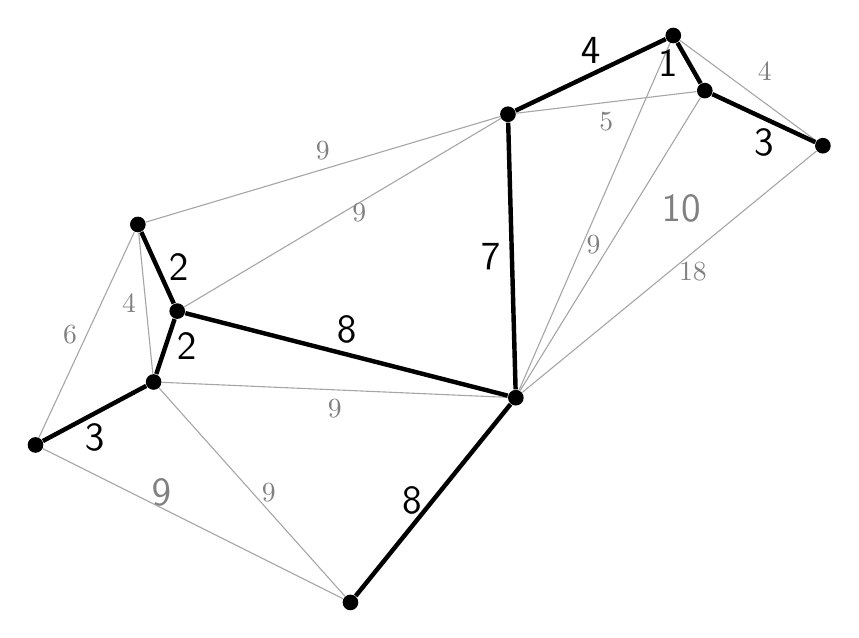
\begin{tikzpicture}[
    node/.style={circle, fill=black, inner sep=2pt},
    thick_edge/.style={ultra thick, draw=black},
    thin_edge/.style={thin, draw=gray!70},
    weight/.style={font=\sffamily\Large}
]

    \node[node] (n1) at (0,2) {};
    \node[node] (n2) at (1.5,2.8) {};
    \node[node] (n3) at (1.3,4.8) {};
    \node[node] (n4) at (1.8,3.7) {};
    \node[node] (n5) at (4,0) {};
    \node[node] (n6) at (6.1,2.6) {};
    \node[node] (n7) at (6,6.2) {};
    \node[node] (n8) at (8.1,7.2) {};
    \node[node] (n9) at (8.5,6.5) {};
    \node[node] (n10) at (10,5.8) {};

    \draw[thin_edge] (n1) -- (n3) node[midway, left, gray] {6};
    \draw[thin_edge] (n2) -- (n3) node[midway, left, gray] {4};
    \node[gray, weight] at (1.6,1.4) {9}; 
    \draw[thin_edge] (n1) -- (n5);
    \draw[thin_edge] (n2) -- (n5) node[midway, right, gray] {9};
    \draw[thin_edge] (n2) -- (n6) node[midway, below, gray] {9};
    \draw[thin_edge] (n3) -- (n7) node[midway, above, gray] {9};
    \draw[thin_edge] (n4) -- (n7) node[midway, right, gray] {9};
    \draw[thin_edge] (n7) -- (n9) node[midway, below, gray] {5};
    \draw[thin_edge] (n8) -- (n10) node[midway, above right, gray] {4};
    \draw[thin_edge] (n6) -- (n9) node[midway, left, gray] {9};
    \draw[thin_edge] (n6) -- (n10) node[midway, right, gray] {18};
    \node[gray, weight] at (8.2,5) {10}; 
    \draw[thin_edge] (n6) -- (n8);

    \draw[thick_edge] (n1) -- (n2) node[midway, below, weight] {3};
    \draw[thick_edge] (n2) -- (n4) node[midway, right, weight] {2};
    \draw[thick_edge] (n3) -- (n4) node[midway, right, weight] {2};
    \draw[thick_edge] (n4) -- (n6) node[midway, above, weight] {8};
    \draw[thick_edge] (n5) -- (n6) node[midway, left, weight] {8};
    \draw[thick_edge] (n6) -- (n7) node[midway, left, weight] {7};
    \draw[thick_edge] (n7) -- (n8) node[midway, above, weight] {4};
    \draw[thick_edge] (n8) -- (n9) node[midway, left, weight] {1};
    \draw[thick_edge] (n9) -- (n10) node[midway, below, weight] {3};
\end{tikzpicture}
\caption{The minimum spanning tree for a planar graph.}
\end{figure}
It is well known that a minimum spanning tree can be computed in polynomial time, for instance using Prim's or Kruskal's algorithm. In contrast, the metric TSP remains NP-hard. Consequently, although an MST connects all vertices at minimum total cost among trees, it does not correspond to a Hamiltonian tour, nor does it necessarily approximate the optimal tour arbitrarily well. Nevertheless, the cost of a minimum spanning tree provides a natural lower bound on the cost of an optimal TSP tour. Indeed, removing any edge from a Hamiltonian cycle yields a spanning tree, implying that
\begin{equation}
    c(\mathrm{MST}) \leq c(\mathrm{OPT}).
\end{equation}
This observation forms the basis of the classical 2-approximation algorithm, which we present in the following section, followed by the 3/2-approximation algorithm of Christofides.

A related problem is the (metric) Steiner tree problem, which seeks a minimum-weight tree that spans a given subset of vertices (called terminals). Like the metric TSP, this problem admits a 2-approximation algorithm based on minimum spanning trees \cite{vazirani}.

\subsection{A simple factor 2 algorithm}
This algorithm is commonly referred to as the \emph{double-tree algorithm}.

\begin{enumerate}
    \item Compute a minimum spanning tree $T$ of $G$.
    \item Double every edge of $T$ to obtain an Eulerian multigraph.
    \item Compute an Eulerian tour $\mathcal{T}$ of this multigraph.
    \item Traverse the vertices in the order of their first appearance in $\mathcal{T}$, shortcutting repeated vertices, and output the resulting Hamiltonian cycle $\mathcal{C}$.
\end{enumerate}

\begin{theorem}
The double-tree algorithm is a $2$-approximation algorithm for the metric TSP.
\end{theorem}

\begin{proof}
Let $c(T)$ denote the cost of the minimum spanning tree. Since removing any edge from an optimal Hamiltonian cycle yields a spanning tree, we have \(c(T) \leq c(\mathrm{OPT})\). After doubling every edge of $T$, the resulting Eulerian multigraph has total cost, i.e. \(c(\mathcal{T}) = 2\,c(T)\). Hence, we have \(c(\mathcal{T}) \leq 2\,c(\mathrm{OPT})\). Finally, by the triangle inequality, shortcutting repeated vertices in the Eulerian tour does not increase the total cost. Therefore, \(c(\mathcal{C}) \leq c(\mathcal{T}) \leq 2\,c(\mathrm{OPT})\), which proves the claim.
\end{proof}

\begin{figure}[htbp]
    \centering
    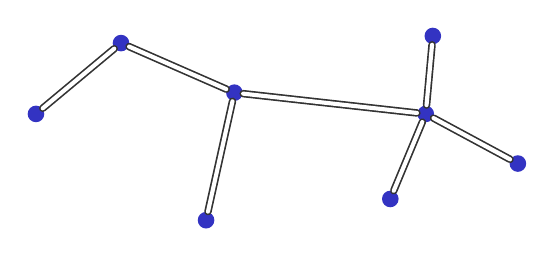
\begin{tikzpicture}[
        atom/.style={
            circle,
            fill=blue!70!black!80,
            minimum size=6pt,
            inner sep=0pt
        },
        bond/.style={
            double,
            double distance=1.5pt,
            line width=0.6pt,
            line cap=round,
            draw=black!80
        },
        scale=0.9
    ]
        % Coordinates
        \node[atom] (n1) at (-2.5, 0.2) {};
        \node[atom] (n2) at (-1.3, 1.2) {};
        \node[atom] (n3) at (0.3, 0.5) {};
        \node[atom] (n4) at (-0.1, -1.3) {};
        \node[atom] (n5) at (3, 0.2) {};
        \node[atom] (n6) at (3.1, 1.3) {};
        \node[atom] (n7) at (2.5, -1) {};
        \node[atom] (n8) at (4.3, -0.5) {};
        
        % Doubled MST edges
        \draw[bond] (n1) -- (n2);
        \draw[bond] (n2) -- (n3);
        \draw[bond] (n3) -- (n4);
        \draw[bond] (n3) -- (n5);
        \draw[bond] (n5) -- (n6);
        \draw[bond] (n5) -- (n7);
        \draw[bond] (n5) -- (n8);
    \end{tikzpicture}
    \caption{Illustration of the double-tree algorithm \cite{traub}: the edges of the minimum spanning tree are doubled to obtain an Eulerian multigraph.}
    \label{fig:double_tree}
\end{figure}
Before we dive into Christofides algorithm, we briefly review perfect matchings.
\subsection{Perfect Matchings}
\begin{definition}
Let $G=(V,E)$ be a graph, a \textit{matching} $M \subseteq E$ is a set of disjoint edges such that at most one edge in $M$ is incident to any node in $V$. A matching is \textit{perfect} if it covers all nodes. The \textit{weight} of a matching is the sum of the weights of the edges in the matching.    
\end{definition}

\begin{figure}[h]
\centering
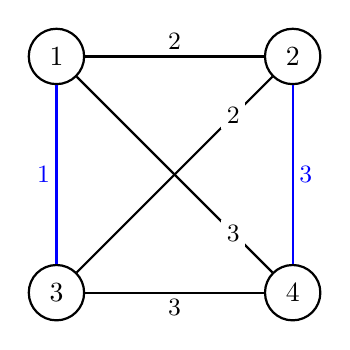
\begin{tikzpicture}[
    node distance={3cm}, 
    vertex/.style = {draw, circle, minimum size=20pt, thick},
    edge_label/.style = {fill=white, inner sep=2pt, font=\small}
] 
    \node[vertex] (1) at (0, 3) {1}; 
    \node[vertex] (2) at (3, 3) {2}; 
    \node[vertex] (3) at (0, 0) {3}; 
    \node[vertex] (4) at (3, 0) {4}; 

    \draw[thick] (1) -- node[edge_label, midway, above] {2} (2); 
    \draw[thick, blue] (1) -- node[edge_label, midway, left] {1} (3); 
    \draw[thick] (3) -- node[edge_label, midway, below] {3} (4); 
    \draw[thick, blue] (2) -- node[edge_label, midway, right] {3} (4); 
    \draw[thick] (1) -- node[edge_label, pos=0.8] {3} (4); 
    \draw[thick] (2) -- node[edge_label, pos=0.2] {2} (3); 
\end{tikzpicture}
    \caption{A minimum weight perfect matching in $K_{4}$, the number of perfect matchings is 3}
\end{figure}

\subsection{Christofides Algorithm}

\begin{enumerate}
    \item Compute a minimum spanning tree $T$ of $G$.
    \item Let $V' \subseteq V$ be the set of vertices of odd degree in $T$. 
          Compute a minimum-cost perfect matching $M$ on $V'$ and add $M$ to $T$. 
          The resulting multigraph is Eulerian.
    \item Compute an Eulerian tour $\mathcal{T}$ of this multigraph.
    \item Shortcut repeated vertices in $\mathcal{T}$ and output the resulting 
          Hamiltonian cycle $\mathcal{C}$.
\end{enumerate}

\begin{theorem}
Christofides algorithm is a $\tfrac{3}{2}$-approximation algorithm for the metric TSP.
\end{theorem}

\begin{proof}
Let $H$ be an optimal TSP tour and denote its cost by $c(\mathrm{OPT})$. As before, removing any edge from $H$ yields a spanning tree, so \( c(T) \leq c(\mathrm{OPT})\). Let $V'$ be the set of vertices of odd degree in $T$. Since every graph contains an even number of odd-degree vertices, $|V'|$ is even, and a perfect matching on $V'$ exists. Consider the tour $H$ and restrict it to the vertices in $V'$ by shortcutting vertices not in $V'$. By the triangle inequality, the resulting tour $H'$ satisfies \(c(H') \leq c(\mathrm{OPT})\). Since $|V'|$ is even, the edges of $H'$ can be partitioned into two perfect matchings $M_1$ and $M_2$, obtained by taking alternating edges along the cycle. Thus,
\[
c(M_1) + c(M_2) = c(H').
\]
Let $M$ be a minimum-cost perfect matching on $V'$. Then
\[
c(M) \leq \min\{c(M_1), c(M_2)\}
      \leq \frac{1}{2} c(H')
      \leq \frac{1}{2} c(\mathrm{OPT}).
\]
The multigraph obtained by adding $M$ to $T$ is Eulerian, and hence its Eulerian tour $\mathcal{T}$ has cost
\[
c(\mathcal{T}) = c(T) + c(M).
\]
Finally, shortcutting repeated vertices does not increase the cost by the triangle inequality, so
\[
c(\mathcal{C}) \leq c(\mathcal{T})
              \leq c(T) + c(M)
              \leq c(\mathrm{OPT}) + \frac{1}{2}c(\mathrm{OPT})
              = \frac{3}{2}c(\mathrm{OPT}),
\]
which completes the proof.
\end{proof}

\begin{figure}[htbp]
    \centering
    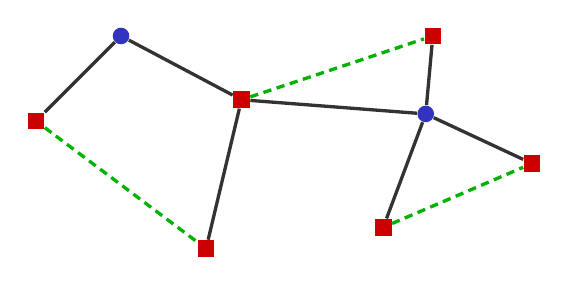
\begin{tikzpicture}[
        blue_node/.style={
            circle,
            fill=blue!70!black!80,
            minimum size=6pt,
            inner sep=0pt
        },
        red_node/.style={
            rectangle,
            fill=red!80!black,
            minimum size=6pt,
            inner sep=0pt
        },
        solid_edge/.style={
            draw=black!80,
            line width=1.2pt
        },
        dashed_edge/.style={
            draw=green!70!black,
            line width=1.2pt,
            dashed,
            dash pattern=on 3pt off 2pt
        },
        scale=0.9
    ]
        % Coordinates
        \node[red_node]  (r1) at (-2.8, 0.1) {};
        \node[blue_node] (b1) at (-1.6, 1.3) {};
        \node[red_node]  (r2) at (0.1, 0.4) {};
        \node[red_node]  (r3) at (-0.4, -1.7) {};
        \node[red_node]  (r4) at (2.8, 1.3) {};
        \node[blue_node] (b2) at (2.7, 0.2) {};
        \node[red_node]  (r5) at (2.1, -1.4) {};
        \node[red_node]  (r6) at (4.2, -0.5) {};

        % MST edges
        \draw[solid_edge] (r1) -- (b1);
        \draw[solid_edge] (b1) -- (r2);
        \draw[solid_edge] (r2) -- (r3);
        \draw[solid_edge] (r2) -- (b2);
        \draw[solid_edge] (b2) -- (r4);
        \draw[solid_edge] (b2) -- (r5);
        \draw[solid_edge] (b2) -- (r6);

        % Matching edges
        \draw[dashed_edge] (r1) -- (r3);
        \draw[dashed_edge] (r2) -- (r4);
        \draw[dashed_edge] (r5) -- (r6);
    \end{tikzpicture}
    \caption{Illustration of the Christofides algorithm \cite{traub}: instead of doubling all edges, a minimum-cost perfect matching is added on the odd-degree vertices (shown in red).}
    \label{fig:christofides}
\end{figure}
The spanning tree is bounded by $c(T) \leq c(\mathrm{OPT})$, while the matching cost is bounded by decomposing the optimal Hamiltonian cycle into two perfect matchings on the odd-degree vertices. Combining these bounds yields the 3/2-approximation guarantee.

\section{Repeated Assignment Heuristic}
\label{RA_heuristic}
The first nontrivial approximation algorithm for the ATSP was developed by Frieze, Galbiati, and Maffioli \cite{frieze1982}, achieving an $O(\log n)$ approximation ratio. This algorithm, commonly known as the \emph{cycle cover algorithm} or \emph{repeated assignment heuristic}, constructs a Hamiltonian cycle through iterative application of minimum-cost assignment problems. A cycle cover of a graph $G=(V,A)$ is a subset $F \subseteq A$ of arcs such that every node has in-degree and out-degree equal to one (i.e., Eulerian) but not necessarily connected. A connected cycle cover would be a Hamiltonian tour and the optimal tour cost would be that of the optimal solution to the assignment problem (AP).

\subsection{Assignment Problem}
Consider a directed graph \(G:=(V\cup\{0\}, A)\) where $\{0\}$ represents the depot node and \(V:=\{1,\dots,n\}\) is the node set. The arc set \(A := \{(i,j) \in (V \cup \{0\})\times(V\cup \{0\}) \mid i \neq j,\ c_{ij} < \infty \}\) contains all available arcs with finite cost $c_{ij} > 0$. It is assumed that the costs satisfy the asymmetric triangle inequality on available arcs, i.e., for any $i,j,k \in V \cup \{0\}$ with \((i,j),(j,k),(i,k) \in A\), \( c_{ik} \leq c_{ij} + c_{jk} \). The assignment problem relaxation of the ATSP is formulated as follows:
\begin{align}
\min \quad & \sum_{(i,j) \in A} c_{ij} x_{ij} \label{eq:ap_obj}\\
\text{s.t.} \quad 
& \sum_{j:(i,j) \in A} x_{ij} = 1 && \forall i \in V \cup \{0\}, \label{eq:ap_out}\\
& \sum_{i:(i,j) \in A} x_{ij} = 1 && \forall j \in V \cup \{0\}, \label{eq:ap_in}\\
& x_{ij} \in \{0,1\}  && \forall (i,j) \in A. \label{eq:ap_binary}
\end{align}
This formulation enforces exactly one outgoing and one incoming arc at each node, which is a necessary but not sufficient condition for a Hamiltonian cycle. The solution is a cycle cover, i.e., a collection of directed disjoint cycles.

\begin{lemma}
\label{Ass_cover}
Let $\mathrm{OPT}$ denote the optimal cost of ATSP and 
$\mathrm{OPT}_{\mathrm{AP}}$ the optimal cost of the assignment problem (or minimum-cost cycle cover). Then \( \mathrm{OPT}_{\mathrm{AP}} \le \mathrm{OPT}\).
\end{lemma}
\begin{proof}
Every Hamiltonian cycle is a feasible solution to the assignment problem. Therefore the assignment problem is a relaxation of ATSP and its optimal cost cannot exceed that of ATSP. 
\end{proof}

\subsection{Algorithm}
\begin{enumerate}
    \item Compute a minimum-cost cycle cover with cycles $C_1, \dots, C_k$ on the node set $V \cup \{0\}$ using the assignment relaxation.
    \item From each $C_i$, select an arbitrary proxy node $v_i$.
    \item Recursively apply the same procedure on the reduced graph containing only the proxy nodes, $G[\{v_1,\dots,v_k\}]$ to obtain a tour $C$.
    \item Combine this with the cycle cover, \(C' = C \cup C_1 \cup C_2 \dots C_k\), to obtain an Eulerian graph $C'$.
    \item Repeated nodes in $C'$ are shortcut, using the triangle inequality to obtain a Hamiltonian cycle $\mathcal{C}$ on $V \cup \{0\}$ that starts and ends at the depot.
\end{enumerate}

\begin{lemma}
Given $G$ satisfies the asymmetric triangle inequality. Then for any \( S \subseteq V \cup \{0\} \), the cost of an optimal TSP tour in $G[S]$ is at most the cost of an optimal TSP tour in $G$. 
\label{sub_bound}
\end{lemma}
\begin{proof}
Let $C$ be an optimal ATSP tour in $G$. Consider the order in which the nodes of $S$ appear along $C$. Since $G$ satisfies the triangle inequality, $C$ can be shortcut to produce another cycle $C'$ with only $S$ nodes and whose cost is at most the cost of $C$.
\end{proof}

\begin{theorem}
The repeated assignment heuristic is a $\log_2 n$-approximation algorithm for ATSP.
\end{theorem}

\begin{proof}
We prove the theorem by induction on $N = |V \cup \{0\}|$, the number of nodes in $G$. If $N \leq 2$, the instance is trivial and the algorithm returns an optimal tour. For $N > 2$, the number of cycles $k$ in the cycle cover is at most $\lfloor N/2 \rfloor$, since each cycle in the cover has at least 2 nodes and they are disjoint. Thus $k \leq \lfloor N/2 \rfloor$. Let $C_1, \dots, C_k$ be the cycles on $V \cup \{0\}$ obtained after solving the assignment relaxation. Let $S=\{v_1, \dots, v_k\}$ be the set of proxy nodes, containing one node arbitrarily selected from each cycle, so $|S| = k \leq \lfloor N/2 \rfloor < N$. Let $\mathrm{OPT}(S)$ be the cost of an optimal tour in $G[S]$. From Lemma \ref{sub_bound}, we have \(\mathrm{OPT}(S) \leq \mathrm{OPT}\). The algorithm recurses on the proxy nodes $S$. Since $|S| < N$, by the inductive hypothesis, the cost of the tour $C$ returned by the recursive call is
\[ 
\mathrm{cost}(C) \leq (\log_2 |S|) \cdot \mathrm{OPT}(S) \leq (\log_2 |S|) \cdot \mathrm{OPT}. 
\] 
Combining $C$ with the original cycle cover gives an Eulerian graph \( C' := C \cup C_1 \cup \dots C_k\), whose cost satisfies 
\[
    \mathrm{cost}(C') \le \mathrm{cost}(C) + \sum_{i=1}^k \mathrm{cost}(C_i) \le \log_2 |S| \cdot \mathrm{OPT} + \mathrm{OPT},
\]
because the cycle cover cost (i.e., $\mathrm{OPT}_{\mathrm{AP}}$) is at most $\mathrm{OPT}$ (Lemma \ref{Ass_cover}). Finally, since shortcutting does not increase the cost and $|S| \le \lfloor N/2 \rfloor$, we have
\[
     \mathrm{cost}(\mathcal{C}) \le \log_2 |S| \cdot \mathrm{OPT} + \mathrm{OPT} \le \log_2 (N/2) \cdot \mathrm{OPT} + \mathrm{OPT} = (\log_2 N) \cdot \mathrm{OPT},
\]
Intuitively, at each recursive step the number of nodes decreases by at least a factor of two, since each cycle contains at least two nodes. Therefore, the number of recursion levels is at most $\log_2 N$, and at each level we incur a cost of at most $\mathrm{OPT}$ from the cycle cover.
\end{proof}

\begin{figure}[h]
    \centering
    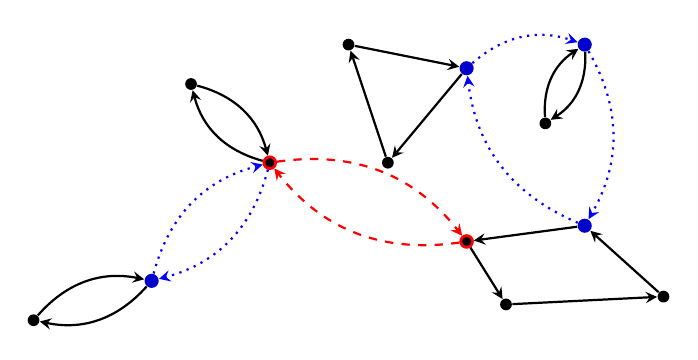
\begin{tikzpicture}[
    node/.style={circle, fill=black, inner sep=1.5pt},
    blue_node/.style={circle, fill=blue!80!black, inner sep=1.8pt},
    red_node/.style={circle, draw=red, fill=black, line width=1pt, inner sep=1.5pt},
    solid_edge/.style={->, thick, >=stealth},
    dotted_edge/.style={->, blue, dotted, thick, >=stealth, bend left},
    dashed_edge/.style={->, red, dashed, thick, >=stealth, bend left}
]

    % --- Nodes ---
    % Left cluster
    \node[node] (n1) at (0,0) {};
    \node[blue_node] (n2) at (1.5,0.5) {};
    
    % Mid-left cluster
    \node[node] (n3) at (2,3) {};
    \node[red_node] (n4) at (3,2) {};
    
    % Top center cluster
    \node[node] (n5) at (4,3.5) {};
    \node[blue_node] (n6) at (5.5,3.2) {};
    \node[node] (n7) at (4.5,2) {};
    
    % Top right cluster
    \node[node] (n8) at (6.5,2.5) {};
    \node[blue_node] (n9) at (7,3.5) {};
    
    % Bottom center cluster
    \node[red_node] (n10) at (5.5,1) {};
    \node[node] (n11) at (6,0.2) {};
    \node[node] (n12) at (8,0.3) {};
    \node[blue_node] (n13) at (7,1.2) {};

    % --- Edges: Iteration 1 (Solid Black) ---
    \draw[solid_edge] (n1) to[bend left] (n2);
    \draw[solid_edge] (n2) to[bend left] (n1);
    
    \draw[solid_edge] (n3) to[bend left] (n4);
    \draw[solid_edge] (n4) to[bend left] (n3);
    
    \draw[solid_edge] (n5) -- (n6);
    \draw[solid_edge] (n6) -- (n7);
    \draw[solid_edge] (n7) -- (n5);
    
    \draw[solid_edge] (n8) to[bend left] (n9);
    \draw[solid_edge] (n9) to[bend left] (n8);
    
    \draw[solid_edge] (n10) -- (n11);
    \draw[solid_edge] (n11) -- (n12);
    \draw[solid_edge] (n12) -- (n13);
    \draw[solid_edge] (n13) -- (n10);

    % --- Edges: Iteration 2 (Blue Dotted) ---
    \draw[dotted_edge] (n2) to (n4);
    \draw[dotted_edge] (n4) to (n2);
    \draw[dotted_edge] (n6) to (n9);
    \draw[dotted_edge] (n9) to (n13);
    \draw[dotted_edge] (n13) to (n6);

    % --- Edges: Iteration 3 (Red Dashed) ---
    \draw[dashed_edge] (n4) to (n10);
    \draw[dashed_edge] (n10) to (n4);

\end{tikzpicture}
    \caption{Illustration of the repeated assignment heuristic \cite{traub}. The first iteration chooses a minimum-cost cycle cover. The second iteration chooses a proxy node from each connected component and adds a minimum-cost cycle cover on these (blue). After two more arcs are added in the third iteration (red), the digraph is connected, and the algorithm terminates.}
    \label{fig:cycle-cover}
\end{figure}

This heuristic can be viewed as iteratively enforcing connectivity on the assignment relaxation without explicitly adding subtour elimination constraints. This approximation factor factor was subsequently improved to $0.999 \log_2 n$ \cite{blaser2002}, $0.842 \log_2 n$ \cite{Kaplan_decomposing} and $0.666 \log_2 n$.\cite{Singh_improved}.

We now discuss the $O(\log n / \log \log n)$-approximation by Asadpour et al.~\cite{asadpour}, which was a major breakthrough result in this field. In contrast to the repeated assignment heuristic, which relies on the assignment relaxation, this algorithm builds upon the Held--Karp relaxation \cite{HK_relaxation} of ATSP. 

The algorithm proceeds in three main stages. First, an optimal solution to the Held--Karp linear programming relaxation is computed. From this fractional solution, a probability distribution over spanning trees of the underlying undirected graph is constructed. A spanning tree is then sampled from this distribution such that it is \emph{thin} with respect to the fractional solution, meaning that its cut structure approximately preserves the LP values. Second, the sampled tree is oriented and augmented to obtain a strongly connected Eulerian multigraph. This augmentation is achieved by solving a minimum-cost circulation problem that balances the in-degree and out-degree at each node. Finally, an Eulerian tour of the resulting multigraph is computed and shortcut using the triangle inequality to obtain a Hamiltonian cycle.

\section{Held--Karp Relaxation}
In this section, we introduce the Held--Karp relaxation \cite{HK_relaxation}, also known as the subtour LP \cite{dfj1954}, which serves as a linear programming relaxation of the ATSP. Let \(V_0 := V \cup \{0\}\) denote the full node set including the depot. The number of nodes in the full node set is, \(|V_0| = n+1\). Given a directed graph \(G:=(V_0, A)\) with $V_0$ as nodes, \(A := \{(i,j) \in V_0\times V_0 \mid i \neq j,\ c_{ij} < \infty \}\) as the arc set. The Held--Karp relaxation is the following linear program:
\begin{align}
\min \quad & \sum_{(u,v) \in A} c(u,v) \, x(u,v) \\[0.3em]
\text{s.t.} \quad
& \sum_{u \in S,\, v \in V_0 \setminus S} x(u,v) \ge 1
&& \forall S \subsetneq V_0,
\label{HK_cut} \\[0.3em]
& \sum_{v \in V_0} x(u,v) = \sum_{v \in V_0} x(v,u) = 1
&& \forall u \in V_0
\label{HK_deg} \\[0.3em]
& x(u,v) \ge 0 && \forall (u,v) \in A.
\end{align}
Constraint~\eqref{HK_cut} ensures that for every subset $S \subsetneq V_0$, there is at least one arc leaving $S$, enforcing global connectivity of the solution. Constraints~\eqref{HK_deg} enforce degree balance at each node, ensuring exactly one incoming and one outgoing arc.

The incidence vector of any Hamiltonian cycle is a feasible solution to the above LP. Therefore, the solution of the above LP provides a \emph{lower bound} on the cost of the optimal ATSP tour. 
\begin{equation}
c(x^*) \le \mathrm{OPT}.
\label{HK_bound}
\end{equation}
It is well-known that an optimal solution $x^*$ to this relaxation can be computed in polynomial time~\cite{asadpour}. Without loss of generality, we assume that $x^*$ is an extreme point of the corresponding polytope.

\section{Thin Spanning Trees}

Let $\vec{T}$ be an orientation of a spanning tree $T$ over the node set $V_0$. In order to obtain a feasible ATSP tour, the oriented tree must be augmented to become Eulerian, i.e., every node must have equal in-degree and out-degree and the graph must be strongly connected.

This problem can be formulated as a minimum-cost circulation (or flow) problem and solved efficiently. If $E_{\text{aug}}$ denotes the set of augmentation arcs, then the cost of the resulting ATSP tour after shortcutting the Eulerian multigraph is
\begin{equation}
    c(\mathrm{ATSP}) = c(\vec{T}) + c(E_{\text{aug}}).
\label{cost}
\end{equation}
Therefore, in order to upper-bound the approximation ratio of the algorithm, one must control both the cost of the sampled tree $\vec{T}$ and the cost of the Eulerian augmentation. The notion of \emph{thinness} precisely captures the property that ensures that the augmentation cost remains small.

\subsection{Symmetrization and the Spanning Tree Polytope}

To construct thin spanning trees, we derive an undirected fractional structure from the optimal Held--Karp solution $x^*$. This is done by symmetrizing $x^*$ to obtain a point in the spanning tree polytope. Define the symmetrized vector $z^* \in \mathbb{R}^{\binom{V_0}{2}}$ by
\begin{equation}
  z^*_{\{u,v\}} := \frac{n}{n+1} \left( x^*_{uv} + x^*_{vu} \right)
\label{symmetrize}  
\end{equation}
The spanning tree polytope $P$ of a graph $(V_0, E)$ is defined by the following inequalities \cite{schrijver_GACO}:
\begin{align}
P = \{ z \in \mathbb{R}^E : \ & \sum_{e \in E} z_e = |V_0|-1, \notag\\
& \sum_{e \in E(S)} z_e \le |S|-1 && \forall S \subseteq V_0 \notag\\
& z_e \ge 0 && \forall e \in E. \}
\label{st_polytope}
\end{align}
Here, $E(S)$ denotes the set of edges with both head and tail in $S \subseteq V_0$. The relative interior of $P$ consists of points that satisfy all these inequalities strictly.

We now verify that the symmetrized vector $z^*$ satisfies these constraints \eqref{st_polytope}. The equality
\[
\sum_{e \in E} z^*_e = |V_0|-1
\]
follows directly from the scaling factor $n/(n+1)$ and the fact that $x^*$ has total degree $2$ at each node. It remains to show that the cut constraints are satisfied strictly. For any nonempty subset $S \subset V_0$, we have
\begin{align}
\sum_{e \in E(S)} z^*_e
&= \frac{1}{2} \left(
\sum_{v \in S} \sum_{u \in V_0} z^*_{\{u,v\}}
- \sum_{\substack{u \in S \\ v \in V_0 \setminus S}} z^*_{\{u,v\}}
\right) \notag \\[0.5em]
&= \frac{n}{2(n+1)} \left(
\sum_{v \in S} \sum_{u \in V_0} \big(x^*_{uv} + x^*_{vu}\big)
- \sum_{\substack{u \in S \\ v \in V_0 \setminus S}} \big(x^*_{uv} + x^*_{vu}\big)
\right).
\label{previous_exp}
\end{align}
Using the degree constraints \eqref{HK_deg}, we have
\begin{equation}
\sum_{v \in S} \sum_{u \in V_0} \big(x^*_{uv} + x^*_{vu}\big) = 2|S|.
\label{degrees_HK}
\end{equation}
Moreover, using the cut constraint \eqref{HK_cut}, we have
\begin{equation}
   \sum_{\substack{u \in S \\ v \in V_0 \setminus S}} \big(x^*_{uv} + x^*_{vu}\big) \ge 2. 
\label{cuts_HK}
\end{equation}
Substituting \eqref{degrees_HK} and \eqref{cuts_HK} into \eqref{previous_exp}, we have
\begin{align}
\sum_{e \in E(S)} z^*_e
&\le \frac{n}{2(n+1)} (2|S| - 2) \notag \\
&= \frac{n}{n+1} (|S| - 1)
< |S| - 1.
\end{align}
Thus, $z^*$ lies in the spanning tree polytope. We now formally define thin trees.

\begin{definition}[Thin trees \cite{asadpour}]
Let $G=(V_0,E)$ be an undirected graph and let $z \in \mathbb{R}^E_{\ge 0}$ 
be a point in the spanning tree polytope. A spanning tree $T$ is called 
$\alpha$-thin with respect to $z$ if for every subset $S \subset V_0$,
\[
|T \cap \delta(S)| \leq \alpha \cdot z(\delta(S)).
\]
Here, $\delta(S)$ denotes the set of edges with exactly one endpoint in $S$. We say that $T$ is $(\alpha,s)$-thin if it is $\alpha$-thin and additionally \(c(T) \leq s \cdot c(x^*)\).
\label{thin_trees}
\end{definition}
Definition \ref{thin_trees} disregards the orientation of arcs and considers the underlying undirected graph. This allows the algorithm to work with the spanning tree polytope, while the orientation is restored later when the tree is augmented to obtain an Eulerian directed multigraph. Thin trees provide the key link between the fractional Held--Karp solution and an integral ATSP tour. The following result shows that constructing a thin tree with bounded cost directly yields a good approximation.

\begin{theorem}[Upper bound \cite{asadpour}]
Let $x^*$ be an optimal solution to the Held-Karp relaxation, and $z^*$ be the symmetrized and scaled down version of $x^*$ \eqref{symmetrize} in the spanning tree polytope. If $T^*$ is an $(\alpha,s)$-thin spanning tree with respect to $z^*$ for some $\alpha$ and $s$, then we can find in polynomial-time a Hamiltonian cycle whose cost is at most
\(
(2\alpha + s)\, c(x^*) \le (2\alpha + s)\, \mathrm{OPT}.
\)
\end{theorem}

\section{Maximum Entropy Sampling}
A natural way to round a fractional vector $x = (x_1,\dots,x_n)$ with $0 \le x_i \le 1$, for each $i$, is to perform \emph{independent randomized rounding}~\cite{independent_rounding}, i.e., each variable $x_i$ is set to $1$ with probability $x_i$ and to $0$ with the remaining probability. This procedure preserves the \emph{marginals}, since $\mathbb{E}[\hat x_i] = x_i$. However, independent rounding ignores the combinatorial structure of the solution. In particular, when applied to the fractional spanning-tree vector $z^*$ it may produce a disconnected graph or directed cycles, thus violating the required tree structure. To avoid this issue we seek a probability distribution over spanning trees that:
\begin{itemize}
\item preserves the edge marginals given by $z^*$, and
\item exhibits negative correlation properties \cite{negative_correlation}.
\end{itemize}
Negative correlation is important because it allows the use of Chernoff-type concentration bounds, which are crucial in proving that the sampled tree is thin with high probability.

Among all distributions over spanning trees that preserve the desired marginals, we consider the one with maximum entropy. Intuitively, this is the ``most random'' distribution consistent with the given marginals. It is well known that maximum entropy distributions subject to linear constraints are exponential distributions \cite{boyd2004convex}. In particular, any set of edge weights $\gamma_e$ defines an exponential distribution over spanning trees of the form
\[
p(T) \propto \exp\!\left(\sum_{e\in T} \gamma_e \right),
\]
for some edge weights $\gamma_e$. Moreover, any such exponential distribution is the maximum entropy distribution corresponding to its induced marginals.

Let $E$ denote the support graph of $z^*$ obtained by disregarding the directions of the arcs. We aim to find weights $\{\tilde{\gamma}_e\}_{e\in E}$ such that the induced distribution
\begin{equation}
\tilde p(T) \propto 
\exp\!\left(\sum_{e\in T} \tilde{\gamma}_e\right),
\end{equation}
approximately preserves the marginals imposed by $z^*$. That is, for every edge $e \in E$,
\begin{equation}
\sum_{T \in \mathcal{T} : e \in T} \tilde p(T)
\le (1+\varepsilon)\, z^*_e,
\end{equation}
for some sufficiently small $\varepsilon > 0$.

The problem of finding the maximum entropy distribution that preserves the marginals can be formulated as a convex optimization problem with exponentially many variables. This can be approximated efficiently using a combinatorial algorithm based on multiplicative weights~\cite{asadpour}.

The goal of this procedure is to produce a spanning tree that is sufficiently thin with respect to the vector $z^*$. Preserving the marginals induced by $z^*$ is crucial for proving the thinness guarantees of the approximation algorithm. Thus, representing $z^*$ as a probability distribution over spanning trees via a maximum-entropy distribution provides a natural way to obtain the desired random tree.

\subsection{Maximum Entropy Distribution}

Let $\mathcal{T}$ denote the set of all spanning trees of 
$G=(V_0,E)$ and let $z$ be a point in the spanning tree polytope $P$. We recall that the entropy of a discrete probability distribution $p$ over $\mathcal{T}$ is defined as
\begin{equation}
H(p) = -\sum_{T \in \mathcal{T}} p(T)\log p(T).
\label{entropy_formula}
\end{equation}
The maximum entropy distribution with marginals $z$ can be obtained by solving the convex program:
\begin{align}
\inf \quad & \sum_{T\in\mathcal T} p(T)\log p(T) \\
\text{s.t.}\quad 
& \sum_{T\ni e} p(T)=z_e && \forall e\in E \\
& \sum_{T\in\mathcal T} p(T)=1 \\
& p(T)\ge0 && \forall T\in\mathcal T .
\end{align}
The objective function is strictly convex and the feasible region is compact, therefore the convex program has a unique optimal solution $p^*(\cdot)$. The value $p^*(T)$ determines the probability of sampling any tree $T$ in the maximum entropy rounding scheme.  

For every $e \in E$, a Lagrange multiplier $\delta_e$ is associated to the constraint corresponding to the marginal $z_e$ and the Lagrange function is defined as
\begin{align}
L(p,\delta) 
&= \sum_{T \in \mathcal{T}} p(T) \log p(T) 
   - \sum_{e \in E} \delta_e \Bigg(\sum_{T \ni e} p(T) - z_e \Bigg) \notag \\
&= \sum_{e \in E} \delta_e z_e 
   + \sum_{T \in \mathcal{T}} \Bigg( p(T) \log p(T) - p(T) \sum_{e \in T} \delta_e \Bigg)
\label{lagrange}
\end{align}
Thus, the Lagrange dual to the convex program is \(\sup_{\delta} \inf_{p \geq 0} L(p,\delta)\).
For every $T \in \mathcal{T}$, $p(T)$ must minimize the convex function
\[
p(T) \log p(T) - p(T) \delta(T),
\]
where, \( \delta(T) = \sum_{e \in T} \delta_e \). Taking partial derivatives with respect to $p(T)$, we get 
\begin{equation}
    p(T) = e^{\delta(T) - 1}
    \label{exp_prob}
\end{equation}
Thus, 
\[
\inf_{p \geq 0} L(p,\delta) = \sum_{e \in E} \delta_{e} z_{e} - \sum_{T \in \mathcal{T}} e^{\delta(T) - 1}
\]
Changing variables \(\gamma_e = \delta_e - \frac{1}{n}\) for $e \in E$, the Lagrange dual becomes,
\begin{equation}
    \sup_{\gamma} \left(1 + \sum_{e \in E} z_e \gamma_e - \sum_{T \in \mathcal{T}} e^{\gamma(T)}  \right)
    \label{lagrange_dual}
\end{equation}
The assumption that $z$ is in the interior of the spanning tree polytope implies that strong duality holds. Also, $z$ can be written as a convex combination of all spanning trees in $\mathcal{T}$ such that the coefficient corresponding to each spanning tree is positive. This means that there is a point $p(.)$ in the interior of the convex program. So, the convex program satisfies the Slater's condition which is a sufficient condition for strong duality to hold for a convex optimization problem \cite{boyd2004convex}. Therefore, if $\gamma^*$ is the optimal solution of \eqref{lagrange_dual},
\begin{equation}
    p^*(T) = e^{\gamma^{*}(T)}
\end{equation}
Thus, solving the Lagrange dual problem yields edge weights $\gamma^*$ that define an exponential distribution over spanning trees. Sampling from this distribution produces trees whose marginals approximately match $z$.

\subsection[Sampling Random Trees]{Sampling a $\lambda$-Random Tree}
Given edge weights $\lambda_e \ge 0$ for $e\in E$, a 
\emph{$\lambda$-random spanning tree} of $G$ is a spanning tree $T$ chosen with probability
\[
\Pr[T] \propto \prod_{e\in T} \lambda_e .
\]
In particular, setting $\lambda_e = e^{\gamma_e}$ shows that sampling from the exponential family distribution
\[
p(T) \propto \exp\!\left(\sum_{e\in T}\gamma_e\right)
\]
is equivalent to sampling a $\lambda$-random spanning tree \cite{asadpour, Kulkarni_sampling}.

\subsubsection*{Sequential Sampling Procedure}
One practical method to sample a $\lambda$-random tree works as follows \cite{Kulkarni_sampling}:
\begin{enumerate}
    \item Order the edges $e_1, \dots, e_m$ of $G$ arbitrarily.
    \item Process each edge sequentially. After the $j$-th edge $e_j$:
    \begin{itemize}
        \item Decide probabilistically whether to include $e_j$ in the final tree.
        \item The inclusion probability $p_j$ equals the probability that $e_j$ is in a $\lambda$-random tree conditioned on the choices pmade for $e_1,\dots,e_{j-1}$.
    \end{itemize}
    \item Continue until all edges are processed; the resulting tree $T$ 
    is a $\lambda$-random tree.
\end{enumerate}
The probability $p_j$ can be computed efficiently by considering a graph $G'$ obtained from $G$ by contracting edges already included and deleting edges already excluded. Therefore, to obtain each~$p_j$, we need to compute the probability $p_{G'}[\lambda,f]$ that some edge $f$ is in a $\lambda$-random tree for a given (multi)graph $G'$. For this computation, we use the Kirchhoff's matrix tree theorem \cite[pp.~50--60]{bollobas2002modern}. 

\subsubsection*{Computing Probabilities via Kirchhoff's matrix tree theorem}

Kirchhoff's matrix tree theorem states that $\sum_{T \in \mathcal{T}} \prod_{e \in T} \lambda_e$ for any graph $G$ is equal to the value of any cofactor of the weighted Laplacian $L$ where
\[
L_{ij} = \begin{cases} -\lambda_e & e = (i,j) \in E \\ \sum_{e \in \delta({i})} \lambda_e & i=j \\ 0 & \mbox{otherwise}. \end{cases}
\]
Using this result, all conditional probabilities $p_j$ can be computed in polynomial time. 

\section{Multiplicative Weights Algorithm}
This combinatorial m efficiently computes edge weights $\tilde \gamma$'s that approximately preserve the marginal probabilities given by $z$ and solve the maximum entropy convex program.

\begin{enumerate}  
    \item Initialize $\gamma = \vec{0}$
    \item While there exists an edge $e \in E$ with
    $q_e(\gamma) > (1+\varepsilon) z_e$:
    \begin{enumerate}
        \item Compute $\delta$ such that defining
        \(
        \gamma'_e := \gamma_e - \delta, \quad 
        \gamma'_f := \gamma_f \;\; \forall f \in E \setminus \{e\},
        \)
        ensures
        \(
        q_e(\gamma') = (1 + \varepsilon/2) z_e.
        \)
        \item Update $\gamma \gets \gamma'$.
    \end{enumerate}
    \item Output \(\tilde \gamma := \gamma\)
\end{enumerate}
Here, $q_e(\gamma)$ is the probability that edge $e$ is included in a spanning tree under the current weights 
\[
q_e(\gamma) := \frac{\sum_{T \ni e} \exp(\gamma(T))}{\sum_{T} \exp(\gamma(T))}, 
\quad \text{where } \gamma(T) := \sum_{f \in T} \gamma_f,
\]
Asadpour et al.~\cite{asadpour} showed that the multiplicative weights algorithm converges in polynomial time and executes at most \[O\left(\frac{1}{\varepsilon} |E|^2 [|V| \log(|V|) - \log(\varepsilon z_{\min})]\right)\] iterations, where \(z_{\min} = 2^{-O(n \log n)}\).

\section{ATSP heuristics}
In this section, we discuss a novel heuristic, which is essentially based on approximation algorithms proposed in the literature \cite{asadpour, christofides1976}, and also discuss some classical heuristics \cite{frieze1982}.
\subsection{A simple heuristic}
\label{lp_guided_mst}
This heuristic is inspired by the approximation algorithms of Asadpour et al.~\cite{asadpour} and Christofides~\cite{christofides1976}. The main idea is to use the fractional solution of the Held--Karp relaxation to guide the construction of spanning trees that are likely to contain edges of a good tour. Held--Karp solution often assigns high fractional values to edges that appear in optimal or near-optimal tours. Biasing the tree construction toward these edges therefore increases the likelihood of obtaining a high-quality tour. To our knowledge, there is no formal worst-case guarantee for this heuristic.

\begin{enumerate}
\item We first solve the Held--Karp relaxation and obtain an optimal fractional solution $x^*$ together with the LP lower bound.
\item From $x^*$ we derive undirected edge weights by symmetrization,
\[
w_{ij} = x^*_{ij} + x^*_{ji}
\]
Edges with larger $w_{ij}$ are interpreted as being more likely to appear in a good tour.
\item We then sample a number of spanning trees (i.e., $2\lceil\log n\rceil$) using a biased version of Kruskal's algorithm. The edge costs are perturbed according to the LP weights,
\[
c'_{ij} = c_{ij}(1-\alpha w_{ij}),
\]
where $\alpha\in[0,1]$ controls the strength of the bias toward edges with high LP support. In our experiments we use $\alpha = 0.5$, which provides a moderate preference for such edges while still preserving the original cost structure.

\item For each sampled tree we perform the following steps:
\begin{enumerate}
    \item Orient the edges to obtain a directed graph.
    \item Compute the degree imbalance at each vertex.
    \item Add a minimum-cost set of arcs to balance the degrees,
    producing an Eulerian directed multigraph.
    \item Compute an Eulerian tour and apply shortcutting (using the triangle inequality) to obtain a Hamiltonian tour.
\end{enumerate}
\item Among all sampled trees we return the tour with the minimum cost.
\end{enumerate}

\subsection{Classical heuristics}
We briefly review some classical heuristics for (A)TSP. Their worst-case performance guarantees have been studied by Frieze et al.~\cite{frieze1982}. For the sake of notation in this section, we consider a digraph \(G= (V,A)\) where $V$ contains all the nodes including the depot. Given a heuristic method $H$, its worst-case ratio $R_n(H)$ for $n$ node problems is given by
\[
R_n(H) = \sup \frac{d(T)}{d(T^*)}, \quad d(T^*)>0.
\]
Here, $T^*$ is a minimum length tour and $T$ is a tour generated by heuristic $H$.

\paragraph{Greedy algorithm}
We preprocess arcs in non-decreasing order of cost. At each step, an arc $(i,j)$ is selected provided that (i) node $i$ has not yet been assigned an outgoing arc, (ii) node $j$ has not yet been assigned an incoming arc, and (iii) the addition of the arc does not form a cycle unless it forms a Hamiltonian cycle. For this heuristic, \(R_n = n/2\).

\paragraph{Nearest neighbor algorithm}
Starting from any arbitrary node (e.g., depot), the algorithm repeatedly moves to the unvisited node that can be reached with minimum cost from the current node. This process continues until all nodes have been visited, after which the cycle is completed by returning to the starting node. For this heuristic, \(R_n = n/2\).

\paragraph{Cheapest insertion algorithm}
Initially, the tour consists of only one node. At a general stage the algorithm maintains a subtour $T$ visiting a set of nodes $C \subseteq V$. A node $k \notin C$ is inserted between two consecutive nodes~$i,j \in T$ so as to minimize the increase in tour cost, \( c_{ik} + c_{kj} - c_{ij}\). This procedure is repeated until all nodes have been inserted. For this heuristic, \( R_n = \Omega(n)\).

\section{Implementation Details}
This section describes our implementation of the $O(\log n / \log \log n)$-approximation algorithm of Asadpour et al.~\cite{asadpour}. We follow Oveis Gharan's lecture notes~\cite{ovgharan2015lec4} for the theoretical background.

\paragraph{Electrical flows and effective resistance.}  
Given a weighted undirected graph $G = (V,E)$ with edge weights $w : E \to \mathbb{R}_{>0}$, we interpret each edge as a resistor of conductance $w(e)$ (resistance $1/w(e)$). An \emph{electrical flow} sending one unit from $s$ to $t$ is the unique flow satisfying Ohm's law: there exist vertex potentials $p : V \to \mathbb{R}$ such that for every edge $e = (u,v)$,
\[
x(e) = w(e) \bigl(p(u) - p(v)\bigr).
\]
Writing $L_G = B^\top W B$ for the weighted Laplacian (where $B$ is the incidence matrix and $W$ the diagonal conductance matrix), the potential vector satisfies $L_G p = b_{s,t}$, so $p = L_G^\dagger b_{s,t}$ where $L_G^\dagger$ is the Moore--Penrose pseudoinverse~\cite{ovgharan2015lec4}.

The \emph{effective resistance} between $s$ and $t$ is the potential difference induced by one unit of flow:
\[
R_{\mathrm{eff}}(s, t) = b_{s,t}^\top L_G^\dagger b_{s,t} = L^\dagger_{ss} + L^\dagger_{tt} - 2 L^\dagger_{st}.
\]
The second equality follows by expanding $(e_s - e_t)^\top L^\dagger (e_s - e_t)$~\cite{ovgharan2015lec4}. In our implementation, the pseudoinverse is computed via eigendecomposition for numerical stability.

\paragraph{Maximum entropy distribution.}
We compute $\gamma_e$'s for each edge $e \in E$ using the multiplicative weights algorithm of Asadpour et al.~\cite{asadpour}. At each iteration, we define weights $\lambda_e = e^{\gamma_e}$ and construct the corresponding weighted Laplacian matrix $L$. Using the connection between spanning tree distributions and electrical flows, the marginal probability that an edge $e = (i,j)$ appears in a $\lambda$-random spanning tree is given by 
\[ 
q_e \;=\; \lambda_e \cdot R_{\mathrm{eff}}(i,j).
\]
where $R_{\mathrm{eff}}(i,j)$ is computed with respect to the Laplacian weighted by $\{\lambda_e\}$. Whenever a marginal $q_e$ exceeds $(1+\varepsilon) z^*_e$, the parameter $\gamma_e$ is decreased by a fixed step \(\delta = \ln(1 + \varepsilon/2)\) to reduce the probability of selecting this edge. The update is \emph{one-sided}, i.e., $\gamma_e$ is only decreased when $q_e$ is too large, and never explicitly increased. The procedure iterates until all edge marginals approximately satisfy their target values.

\paragraph{Sampling $\lambda$-random spanning trees.}  
With $\gamma_e$ fixed, spanning trees are sampled according to
\[
\Pr(T) \propto \prod_{e \in T} \lambda_e.
\]
Enumerating all spanning trees is infeasible, so we use stochastic procedures.

\paragraph{Contraction-based sequential sampling} Edges are processed in random order. For each edge $e$ still present in the contracted graph, its inclusion probability $q_e$ is computed from the Laplacian pseudoinverse. The edge is added to the tree with probability $q_e$, and the graph is contracted; otherwise, it is discarded. If fewer than $n-1$ edges are selected due to numerical issues, the partial tree is completed greedily using the remaining highest-weight edges.

\paragraph{Gumbel--Kruskal} If the contraction sampler fails, we draw independent Gumbel variables $g_e$ for each edge and compute 
\[ 
s_e = \log \lambda_e + g_e.
\]
A Kruskal-like algorithm processes edges in decreasing order of $s_e$, producing a spanning tree sampled exactly from the $\lambda$-random distribution~\cite{maddison2015asampling}.

\paragraph{Multiple samples and tour selection.}  
We independently sample $k = 2 \lceil \ln n \rceil$ trees~\cite{asadpour} and construct tours from each. The tour with minimum total cost is returned as the final solution.

\section{Computational Experiments}
The approximation algorithms described in this chapter \cite{asadpour, frieze1982}, along with the heuristic described in Section~\ref{lp_guided_mst} are implemented in Python. All experiments run on a laptop with a 13th Gen Intel(R) Core(TM) i7-1355U(12) 5Ghz processor running Arch Linux on linux 6.18.9-arch1-2 kernel. Table~\ref{tab:summary} summarizes the results obtained by running all the algorithms on the 500 sampled routes~\cite{data}, and reports which algorithm performed the best, for how many instances, number of time windows violated, time-window feasible routes and the runtimes. Figure~\ref{fig:nodesvstraveltimes}--\ref{fig:nodesvsruntime} compares the performance of all the algorithms based on the tour costs and computational time. Figure~\ref{fig:marginalverifications} shows that the multiplicative weights procedure (with $\varepsilon=0.2$) achieves marginal convergence quality above 80\% for most instances, which is necessary in proving the worst-case guarantee.

%% figures
\begin{figure}
    \centering 
    \includegraphics[scale=0.45]{images/03_tour_cost_vs_nodes.png} 
    \caption{Travel times comparisons for all the algorithms covered in this chapter.}
    \label{fig:nodesvstraveltimes}
\end{figure}

\begin{figure}[htbp]
    \centering
    \begin{subfigure}{0.48\textwidth}
        \centering
        \includegraphics[scale=0.36]{images/04_runtime_vs_nodes.png}
        \caption{Runtime comparisons of all the algorithms.}
        \label{fig:nodesvsruntime}
    \end{subfigure}
    \hfill
    \begin{subfigure}{0.45\textwidth}
        \centering
        \includegraphics[scale=0.37]{images/06_marginals_vs_nodes.png}
        \caption{Proportion of edges satisfying marginal convergence criterion $|q(e) - z^*(e)|/z^*(e) \leq 0.20$.}
        \label{fig:marginalverifications}
    \end{subfigure}
    
    \vspace{0.5cm}
    
    \begin{subfigure}{0.5\textwidth}
        \centering
        \includegraphics[width=\linewidth]{images/07_repeated_assignment_ratio.png}
        \caption{Performance of the repeated assignment heuristic~\cite{frieze1982} with respect to the assignment relaxation lower bound.}
    \end{subfigure}
    \hfill
    \begin{subfigure}{0.48\textwidth}
        \centering
        \includegraphics[width=\linewidth]{images/08_hk_performance_ratios.png}
        \caption{Performance comparison of heuristic \ref{lp_guided_mst} vs Asadpour et al.~\cite{asadpour} approximation algorithm with respect to the Held--Karp relaxation lower bound.}
        \label{asadpourvsheuristic}
    \end{subfigure}
    
    \caption{}
    \label{fig:}
\end{figure}

\begin{table}[htbp]
\centering
\small
\begin{tabular}{lrrrr}
\toprule
\textbf{Algorithm} & \textbf{Best Tours} & \textbf{TW Sat/Vio} & \textbf{TW Infeas.} & \textbf{Avg. Runtime (s)} \\
\midrule
Cheapest Insertion      & 240 & 5912/568 & 193 & 0.193 \\
Asadpour et al.         & 208 & 5927/553 & 201 & 10.12 \\
Heuristic (Sec.~\ref{lp_guided_mst}) & 30 & 5916/564 & 191 & 3.75 \\
Greedy                  & 15  & 5610/870 & 268 & 0.014 \\
Nearest Neighbor        & 7   & 5940/540 & 204 & 0.002 \\
Repeated Assignment     & 0   & 5940/540 & 204 & 0.019 \\
\bottomrule
\end{tabular}
\caption{Summary of computational results on 500 delivery routes.}
\label{tab:summary}
\end{table}

Overall, the cheapest insertion and Asadpour et al. algorithms dominate in terms of solution quality, with cheapest insertion producing the largest number of best tours. Our heuristic provides a competitive trade-off between runtime and solution quality, outperforming simpler heuristics such as greedy and nearest neighbor. However, Figure~\ref{asadpourvsheuristic} shows that our heuristic consistently produces worse solutions in comparison to the $O(\log n / \log \log n)$-approximation algorithm of Asadpour et al., although it achieves significantly lower runtimes. This highlights a clear trade-off between the running times and the solution quality.  

\begin{table}[ht]
\centering
\small
\begin{tabular}{lrrrrrr}
\toprule
Algorithm & Mean & Median & Std & Min & Max & Lower bound \\
\midrule
Heuristic (Sec. \ref{lp_guided_mst}) & 1.1413 & 1.1384 & 0.0382 & 1.0538 & 1.2790 & Held--Karp relaxation \\
Asadpour et al. & 1.1186 & 1.1193 & 0.0484 & 1.0000 & 1.2455 & Held--Karp relaxation \\
Repeated Assignment & 1.4043 & 1.4051 & 0.1302 & 1.0486 & 1.7381 & Assignment relaxation \\
\bottomrule
\end{tabular}
\caption{Performance ratios across algorithms.}
\label{tab:performance_ratios}
\end{table}

\section{Discussion}
In this chapter, we studied various approximation algorithms proposed in the literature~\cite{asadpour, frieze1982} and implemented them for the asymmetric traveling salesman problem and compared the quality of solutions produced by them on 500 last-mile instances~\cite{data}. We also developed a simple heuristic, based on ideas of Christofides~\cite{christofides1976} and Asadpour et al.~\cite{asadpour}, making use of the optimal solution to the Held--Karp relaxation~\cite{HK_relaxation}, which finds reasonably good solutions. Overall, all the algorithms provided much better solutions than their worst-case guarantees, highlighting the gap between theoretical worst-case analysis and empirical performance on structured instances such as last-mile instances. While time-window constraints were not considered in this chapter, future work could extend our heuristic to handle them, drawing inspiration from Chekuri and Korula~\cite{chekuriTW}, who study approximation algorithms for orienteering with time windows. Additionally, recent advances in approximation algorithms, e.g., Behrendt et al.~\cite{behrendt2020generalizing}, which generalizes the double tree and the Christofides algorithm for the asymmetric setting by parametrization, may provide valuable insights for further improving heuristic performance on asymmetric instances.

\vfill
\section*{Authorship}
This chapter was written by Prajeet Pushkar.

\bibliographystyle{plain}
\bibliography{references}
\end{document}
